\documentclass[a4paper, 14pt]{article}
\usepackage[dvipsnames]{xcolor}
\usepackage[top=70pt,bottom=70pt,left=48pt,right=46pt]{geometry}
\definecolor{header}{RGB}{92,184,92}
\definecolor{defenition}{RGB}{217,83,79}
\definecolor{main_title}{RGB}{66,139,202}
\definecolor{sub_header}{RGB}{91,192,222}
\usepackage[english, russian]{babel}
\usepackage[utf8]{inputenc}
\usepackage{amsmath}
\usepackage{listings}
\usepackage{graphicx}
\usepackage{amsmath}
\title{\textcolor{main_title}{Определение ширины запрещенной зоны полупроводников по спектральной зависимости собственной фотопроводимости}}
\author{Шмаков Владимир Евгеньевич - ФФКЭ гр. Б04-105}






\begin{document}
\maketitle



\section*{\textcolor{header}{Цель работы}}

    Определение ширины запрещённой зоны различных материалов по спектральной зависимости собственной фотопроводимости;


\section*{\textcolor{header}{Теоретические сведения}}
При воздействии на полупроводник излучения с энергией кванта $h\nu$, превышающей ширину запрещённой зоны $E_g$ в зоне проводимости, и соотвественно в валентной зоне возникают неравновесные электроны и дырки. Их появление связано с переходами электронов из валентной зоны проводимости. В результате увеличивается проводимость кристалла. Это явление называется собственной фотопроводимостью.

В непрямозонных полупроводниках типа германия и кремния минимум зоны проводимости и максимум валентной зоны расположены в различных точках зоны Бриллюэна. В этом случае оптический переход электрона из вершины валентной зоны в минимум зоны проводимости возможен лишь при участии третьей частицы – фонона. В соответствии с законом сохранения импульса квазиимпульс такого фонона $q_{\text{ф}}\approx\hbar k_{\text{Б}}$, а энергия $\hbar\omega$ должна удовлетворять закону сохранения энергии:
\begin{equation}
    h\nu = E_g\pm \hbar\omega_q+\hbar^2(k_n-k_c)^2/2m_n+\hbar^2k_p^2/2m_p
\end{equation}
где $k_n$ и $k_p$ -- начальные волновые числа электрона и дырки, а $k_c$ -- конечное волновое число электрона.

Таким образом, край основной полосы поглощения в полупроводниках типа кремния и германия определяется непрямыми оптическими переходами, сопровождающимися поглощением и испусканием фононов. При этом для разрешённых переходов, которые доминируют в полупроводниках такого типа, коэффициент поглощения:

\begin{equation}
    K=C\left[\frac{(h\nu-E_g+\hbar\omega_q)^2}{\exp{\frac{\hbar\omega_q}{kT}}-1}+\frac{(h\nu-E_g-\hbar\omega_q)^2}{1-\exp{-\frac{\hbar\omega_q}{kT}}}\right]
\end{equation}
При больших энергиях квантов $h\nu>(E_g+\hbar\omega_q)$ начинают преобладать переходы с эмиссией фононов и зависимость $K^{1/2}$ от $h\nu$ должна аппроксимироваться прямой, пересекающей ось энергии в точке $h\nu_1=E_g+\hbar\omega_q$.

При рассмотрении случая сильного поглощения излечения в образце (оптически толстый образец), то есть при $d/K<<1$, где $d$ -- толщина образца, скорость генерации электронно-дырочных пар экспоненциально уменьшается от поверхности вглубь образца:
\begin{equation}
    g(x)\approx K(1-R)N_0\exp{-Kx}
\end{equation}
где $R$ -- коэффициент отражения света, а $N_0$ -- поток квантов на единицу поверхности.

Неоднородная германия электронов и дырок в направлении освещения приводит к появлению диффузионно-дрейфовых потоков носителей заряда: быстро диффундирующие носители (электроны) опережают медленные (дырки), что приводит к возникновению электрического поля, ускоряющего медленные носители и замедляющего быстрые и к появлению дрейфовых составляющих потоков. При этом изменение проводимости $\Delta\Sigma$ существенным образом зависит от граничных условий на поверхности образца:
\begin{equation}
    \Delta\Sigma\sim N_0\left(1+\frac{S}{D}\frac{1}{K}\right)
\end{equation}
где $S$ -- скорость поверхностной рекомбинации, $D$ -- коэффициент амбиполярной диффузии.


\section*{\textcolor{header}{Методика}}
\subsection*{\textcolor{sub_header}{Экспериментальная установка}}

Для изменения фотоответа полупроводника $\Delta\Sigma$ образец включается последовательно с нагрузочным сопротивлением и источником постоянного напряжения. При освещении проводимость образца возрастает, происходит перераспределение напряжение между образцом и нагрузкой. В результате падение напряжения $U$ на образце при малом относительном увеличении проводимости уменьшается на величину
    \begin{equation}
        \Delta U=\varepsilon\frac{R_H\cdot R_0^2}{(R_H+R_0)^2}\Delta\Sigma
        \label{eq:deltaU}
    \end{equation}
    где $\varepsilon$ -- постоянное напряжение, $R_H$ и $R_0$ -- сопротивление нагрузки и образца, $\Sigma$ -- проводимость.

    Для повышения чувствительности измерения обычно проводят при периодическом прерывании светового потока. При этом соотношение (\ref{eq:deltaU}) характеризует амплитуду отрицательных импульсов напряжения на концах образца. Для исследования интересующих нас зависимостей $\Delta\Sigma/N_0$ от энергии кванта $h\nu$ наряду с $\Delta U$ необходимо знать спектральное распределение интенсивности источника излучения $N_0(h\nu)$.
    \begin{figure}[!htb]
        \centering
        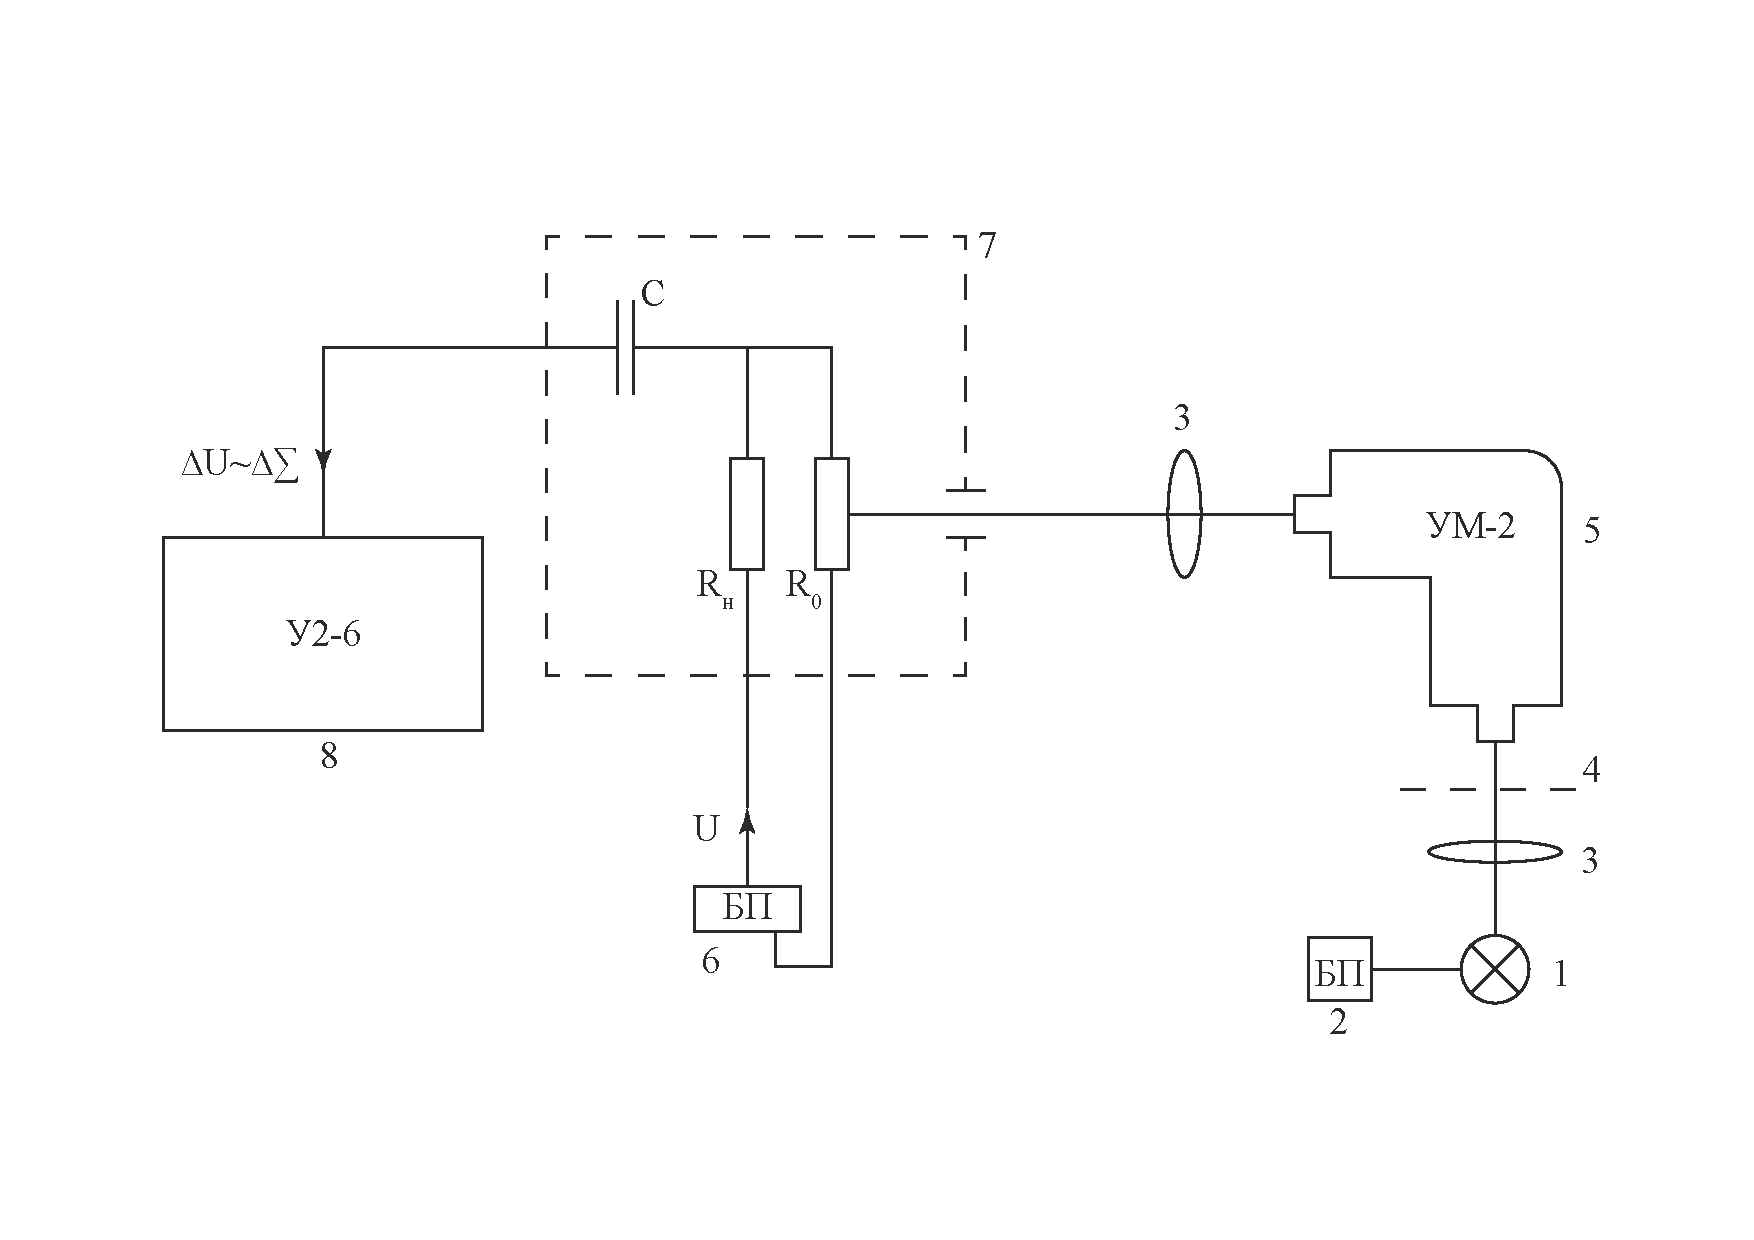
\includegraphics[width=\textwidth]{exp_scheme.pdf}
        \caption{Схема экспериментальной установки. 1 -- осветитель, 2 -- блок питания осветителя, 3 -- линзы, 4 -- механический модулятор излучения, 5 -- монохроматор, 6 -- блок питания образца, 7 -- схема включения образца, 8 -- усилитель}
    \end{figure}

\newpage
\section*{\textcolor{header}{Обработка экспериментальных данных}}

Экспериментальные данные представлены на рисунках $\ref{fig:raw1}$, $\ref{fig:raw2}$.
\begin{figure}[htbp]
    \centering
    \includegraphics*[width = 0.99\textwidth]{CdSe.png}


    \caption{Экспериментальные данне Селен}
    \label{fig:raw1}
\end{figure}

\begin{figure}[htbp]
    \centering
    \includegraphics*[width = 0.99\textwidth]{Ge.png}
    

    \caption{Экспериментальные данне Германий}
    \label{fig:raw2}
\end{figure}


\begin{figure}[htbp]
    \centering
    \includegraphics*[width = 0.5\textwidth]{Si.png}

    

    \caption{Оценка характеристики кремния}
    \label{fig:Si}
\end{figure}
Данные эксперимента с германием позволяют оценить спектральную характеристику для Кремния.
Поделив данные полученные без фильтра на данные, полученные с фильтров получим функцию пропускания(характеристику для кремния).


Построив зависимость квадрата фотоответа от величины энергии кванта можно оценить ширину запрещенной зоны.


\begin{figure}[htbp]
    \centering
    \includegraphics*[width = 0.99\textwidth]{CdSe_power.png}


    \caption{Нахождение ширины запрещенной зоны Селен}
    \label{fig:pow1}
\end{figure}

\begin{figure}[htbp]
    \centering
    \includegraphics*[width = 0.99\textwidth]{Ge_power.png}
    

    \caption{Нахождение ширины запрещенной зоны германий}
    \label{fig:pow2}
\end{figure}

\newpage
\section*{\textcolor{header}{Вывод}}

Удалось найти ширину запрещенной зоны германия и селена. Полученные результаты сходятся с табличными значениями.




\end{document}
